\subsection{Central Time-Of-Flight (CTOF)}

\subsection{Geometry}

The CLAS12 CTOF paddles and light guides, see \F{ctofGeometry} top, are imported from the engineering model. The Step files are converted to tessellated STL files and imported
directly into the GEMC simulation \cite{gemcCad}. The STL files are downloaded using the java geometry service, as the same files are used in reconstruction.
The paddles are assigned the scintillator material and associated with the CTOF hit process routine.
The light guides are also associated to the scintillator material, but they are treated as passive material and not associated with a sensitive detector.

Each volume is typically tessellated by about 1,000 facets. The simulation geometry captures complicated details such as the shape of the scintillator/light guide
junctions, see \F{ctofGeometry} bottom.

\begin{figure}
	\centering
	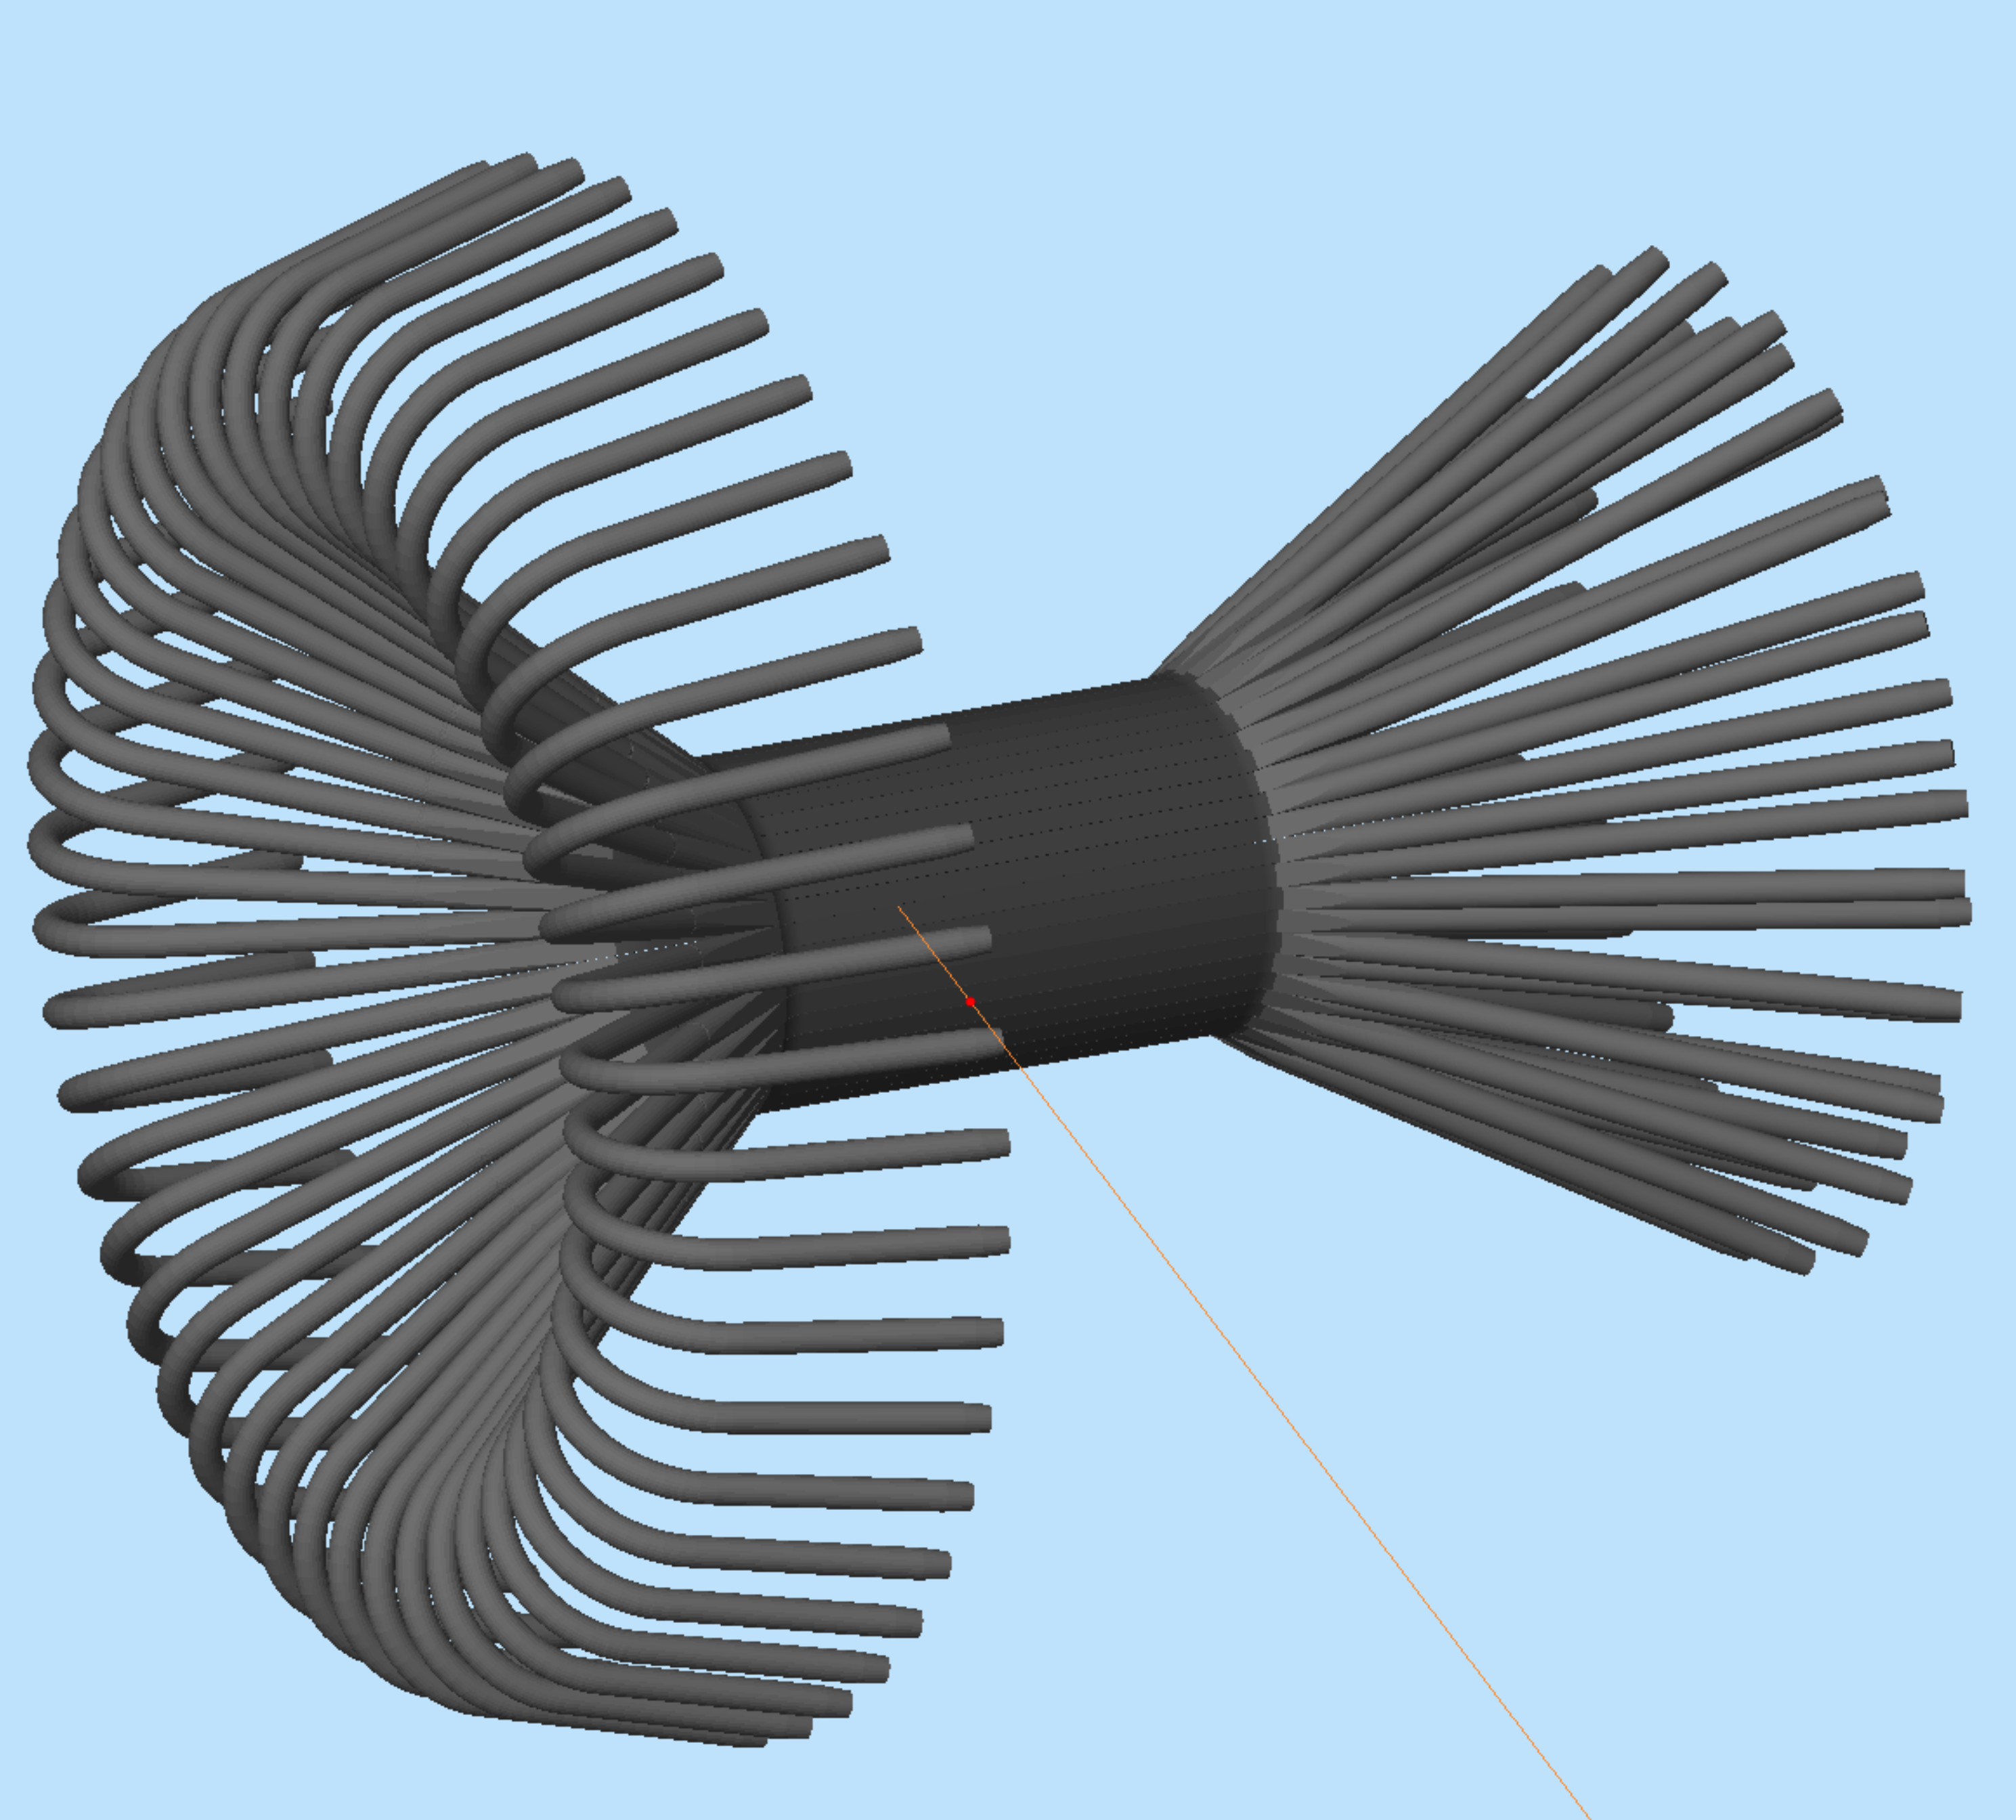
\includegraphics[width=0.99\columnwidth,keepaspectratio]{img/ctofGeometry.png}
	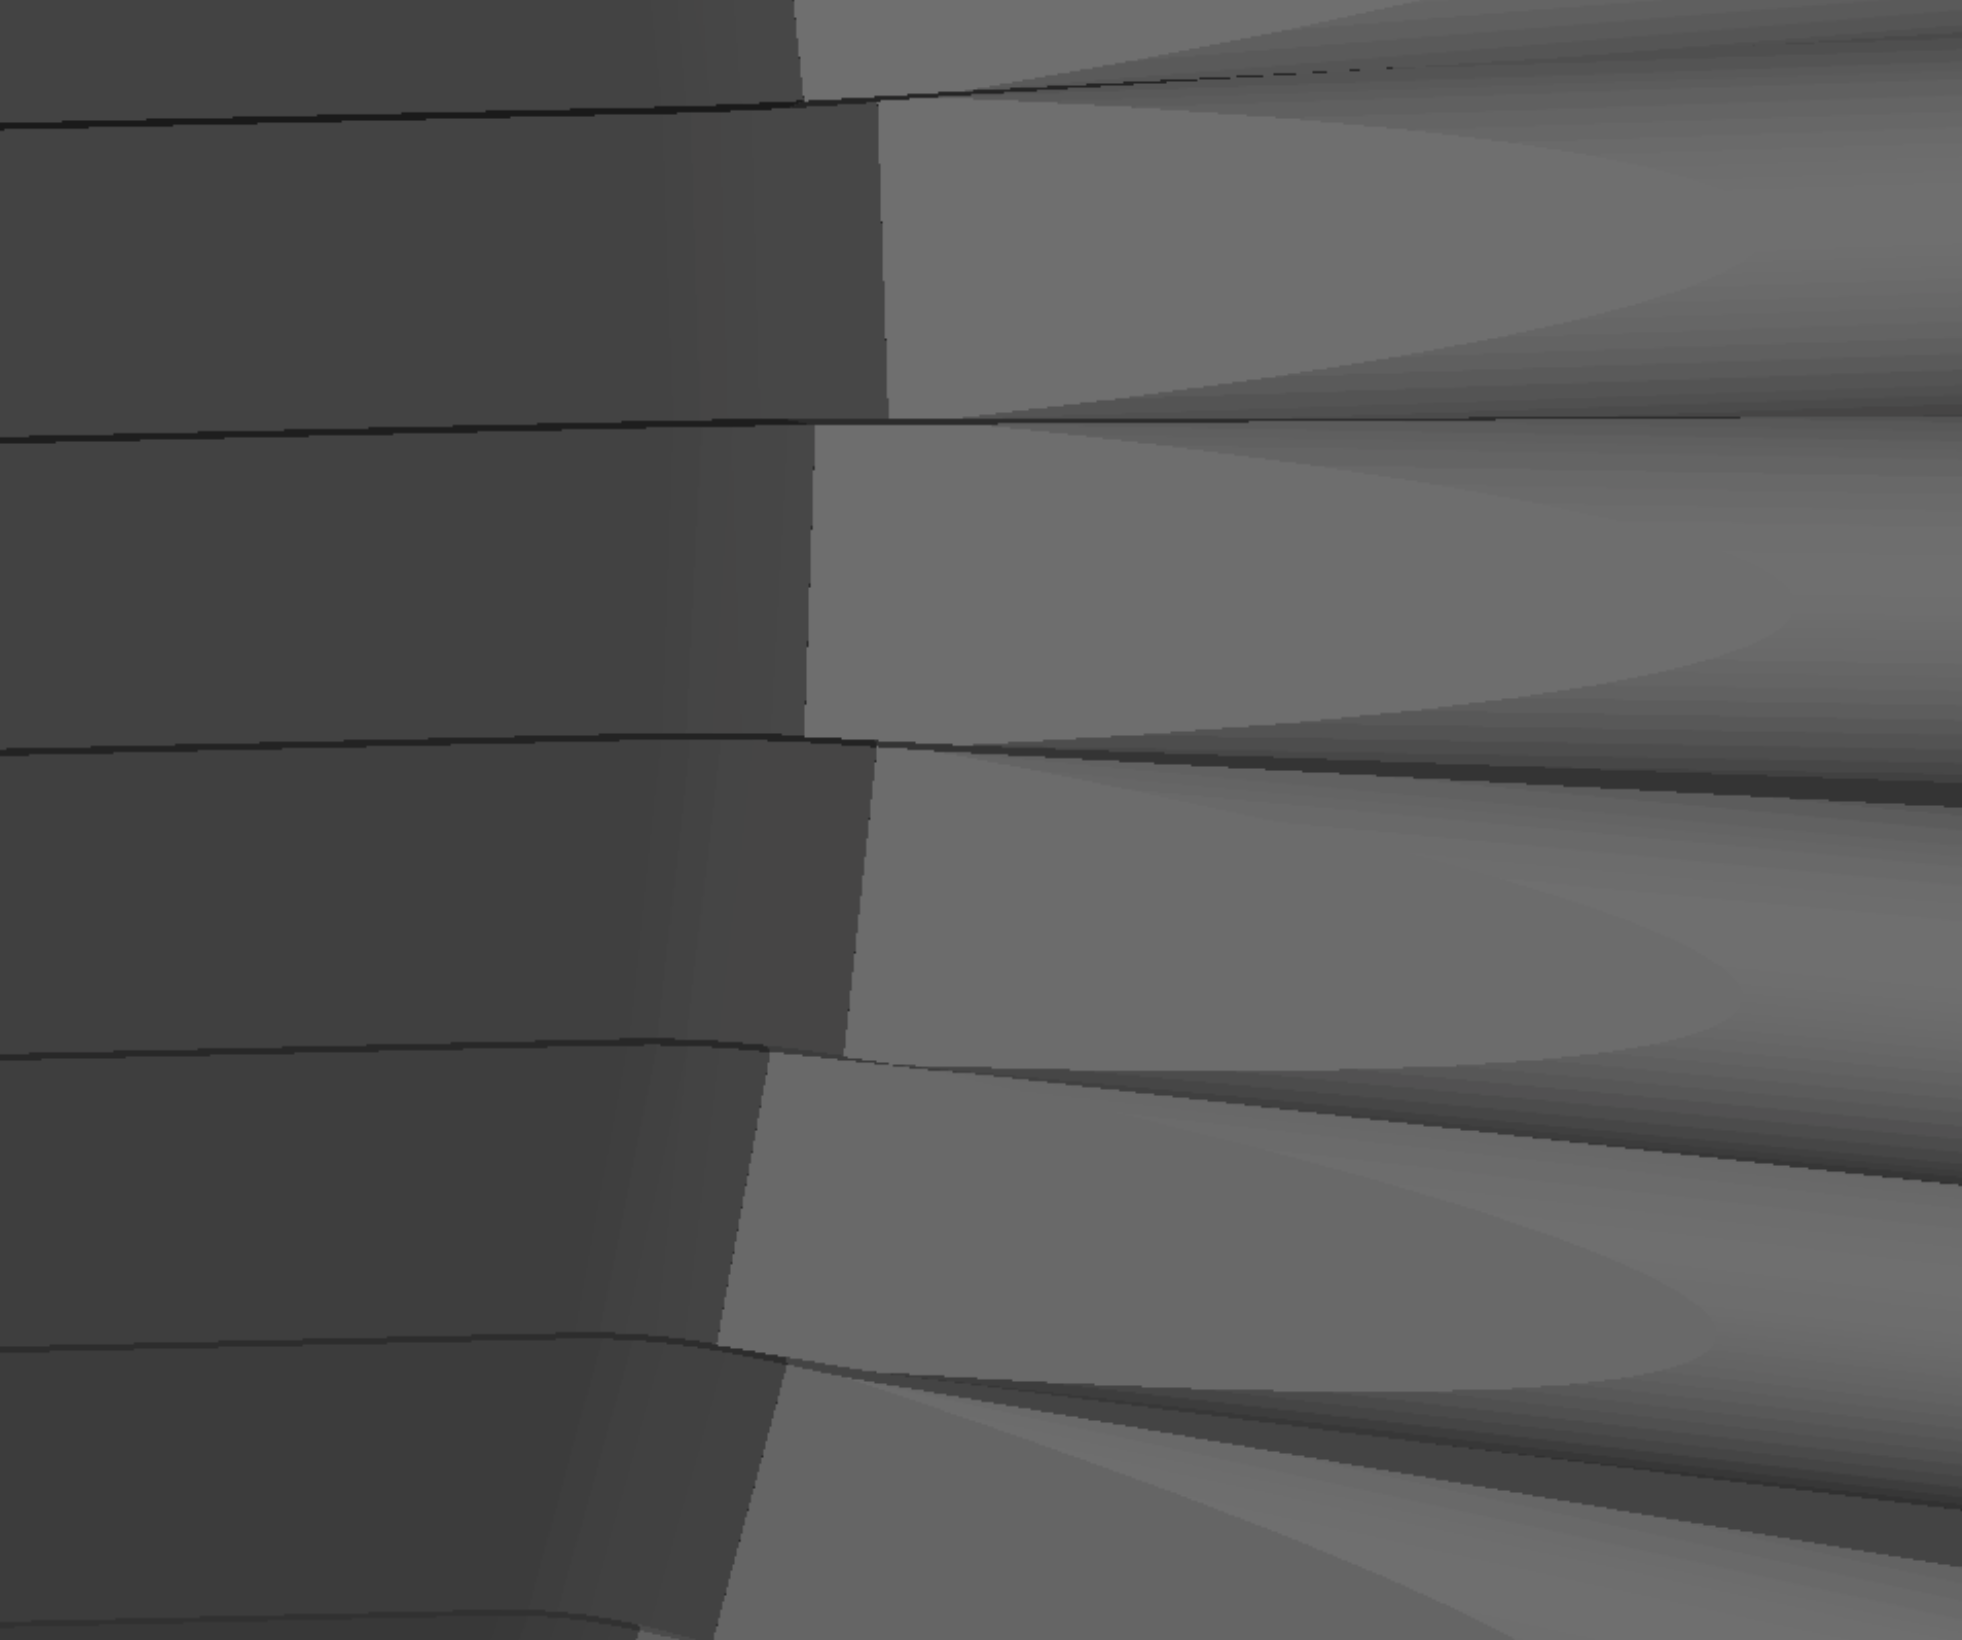
\includegraphics[width=0.99\columnwidth,keepaspectratio]{img/ctofDetail.png}
	\caption{Top: the GEMC implementation of the CTOF geometry. The paddles and light guides are imported directly from the engineering model.
			 The black line is a 2 GeV proton leaving a hit (white circle) in one of the paddles.
			 Bottom: a zoom-in of the implementation shows the details of downstream scintillator/light guide junctions:
			 the scintillator bend near the junction, the light guide starting with a a rectangular shape, and morphing into a circular cross section.}
	\label{fig:ctofGeometry}
\end{figure}

The Github location of the GEMC perl API script is \url{https://github.com/gemc/detectors/tree/master/clas12/ctof}.
The java geometry service is at
\url{https://github.com/JeffersonLab/clas12-offline-software/blob/development/common-tools/clas-jcsg/src/main/java/org/jlab/detector/geant4/v2/CTOFGeant4Factory.java}

\subsection{Process ID}

Each hit in the paddles produces two hits with the identifier variable ``side'' set to 0 (for the upstream PMT) and 1 (for downstream PMT).
The hits are then processed independently through the CTOF hit process routine.

\subsection{Digitization}


The energy deposited is reduced based on the hit position on the paddle using the calibrated attenuation length. It is then corrected by a gain factor
to account for the fact that the HV are adjusted so that the geometric (upstream*downstream) ADC mean sqrt(ADCU*ADCD) is independent of hit position.

The corrected energy is converted to the data derived number of photons $N_{th}$ using the constant $500 \gamma$ / MeV. A Poissonian is used to
calculate the actual number of photons $N_{actual}$ and the resulting ``smeared`` energy is converted to ADC using the FADC conversion factor.


The absolute hit time is corrected by:

\begin{itemize}
	\item the effective velocity (from CCDB)
	\item an upstream/downstream PMT time offset factor (from CCDB)
	\item an RF correction (from CCDB)
\end{itemize}

The time is then smeared by a resolution read from CCDB using a Gaussian function and then digitized using a TDC conversion factor.

The digitized output bank variables are summarized in Table \ref{tab:ctofBank}.

\begin{table}[h]
	\begin{center}
		\begin{tabular}{| c | c | c |}
			\hline \hline
			Variable         & Description   \\
			\hline
              sector  &                             sector number   \\
               layer  &                                     layer   \\
              paddle  &                             paddle number   \\
                side  &                  0 upstream, 1 downstream   \\
                 ADC  &                                       ADC   \\
                 TDC  &                                       TDC   \\
                ADCu  &                             ADC unsmeared   \\
                TDCu  &                             TDC unsmeared   \\
                hitn  &                                hit number   \\
			\hline \hline
		\end{tabular}
	\end{center}
	\caption{The digitized CTOF bank.}\label{tab:ctofBank}
\end{table}

The CTOF hit process routine location in git is \url{https://github.com/gemc/source/blob/master/hitprocess/clas12/ctof_hitprocess.cc}

The time window  of the CTOF is set to to 400 ns: all geant4 steps within the same paddle and time window will be collected on one hit.
